\documentclass[11pt,a4paper,fontset=fandol]{ctexart}

% ====== 版面 ======
\usepackage{geometry}
\geometry{a4paper, left=2.2cm, right=2.2cm, top=2.2cm, bottom=2.2cm, headheight=14pt}
\usepackage{setspace}
\linespread{1.18}
\usepackage{indentfirst}
\setlength{\parindent}{2em}
\emergencystretch=2em

% ====== 颜色 ======
\usepackage{xcolor}
\definecolor{themecolor}{RGB}{40,90,140}
\definecolor{codebg}{RGB}{248,248,245}

% ====== 图、表、数学 ======
\usepackage{graphicx}
\graphicspath{{results/}}
\usepackage{amsmath}
\usepackage{booktabs}
\usepackage{multirow}
\usepackage{caption}
\captionsetup{font=small,labelfont={bf,color=themecolor}}
\usepackage{subcaption}
\usepackage{float}
\usepackage{verbatim}

% ====== 链接 ======
\usepackage{hyperref}
\hypersetup{
  colorlinks=true,
  linkcolor=themecolor,
  citecolor=themecolor,
  urlcolor=themecolor!70!black,
}

% ====== 章节样式：主题色 + 横线分割 ======
\usepackage{titlesec}
\titleformat{\section}
  {\color{themecolor}\bfseries\fontsize{13}{16}\selectfont}
  {\thesection}{0.6em}{}[\vspace{-0.35em}{\color{themecolor!55}\hrule height 0.4pt}]
\titlespacing*{\section}{0pt}{1.0em}{0.4em}

\titleformat{\subsection}
  {\color{themecolor!85!black}\bfseries\fontsize{11.5}{14}\selectfont}
  {\thesubsection}{0.6em}{}
\titlespacing*{\subsection}{0pt}{0.6em}{0.2em}

\titleformat{\subsubsection}
  {\bfseries\fontsize{10.5}{13}\selectfont}
  {\thesubsubsection}{0.6em}{}
\titlespacing*{\subsubsection}{0pt}{0.5em}{0.2em}

% ====== 页眉页脚 ======
\usepackage{fancyhdr}
\pagestyle{fancy}
\fancyhf{}
\renewcommand{\headrulewidth}{0.4pt}
\lhead{\small\color{black!55} ROS 通信机制实验报告}
\rhead{\small\color{black!55} 人工智能 2302}
\cfoot{\small\color{black!55}\thepage}

\fancypagestyle{plain}{
  \fancyhf{}
  \renewcommand{\headrulewidth}{0pt}
  \cfoot{\small\color{black!55}\thepage}
}

% ====== 代码块加浅色边框 ======
\usepackage{mdframed}
\BeforeBeginEnvironment{verbatim}{
  \begin{mdframed}[
    backgroundcolor=codebg,
    linecolor=themecolor!30,
    linewidth=0.5pt,
    innerleftmargin=10pt,
    innerrightmargin=8pt,
    innertopmargin=6pt,
    innerbottommargin=4pt,
    skipabove=8pt,
    skipbelow=8pt,
    roundcorner=2pt,
  ]
}
\AfterEndEnvironment{verbatim}{\end{mdframed}}

\setCJKmonofont{Arial Unicode MS}

% ====== 标题页信息 ======
\title{\bfseries ROS 通信机制实验报告}
\author{人工智能2302 \quad 蒋梓轩\\
人工智能2302 \quad 汪翌秦\\
人工智能2302 \quad 孙靖淞}
\date{2026 年 4 月 28 日}

\begin{document}

\maketitle

\section{实验目的}

本次实验围绕 ROS Noetic 中两种最常见的通信方式——话题（Topic）和服务（Service）展开，希望通过自己实现节点、运行节点、再用工具观察节点之间的交互，建立起对 ROS 计算图的直观理解。在 ROS 里，机器人系统通常被拆成多个职责单一的节点，节点之间不直接调用对方函数，而是依靠 ROS Master 的注册机制完成对接。这种"分布式 + 解耦"的设计是后续学习感知、规划、控制等模块的基础，因此本次实验的目标就是把这套机制从概念落实到可运行的代码上。

具体来说，实验分三块内容。第一块是话题通信，需要写一个以固定频率发送字符串的发布者，再用一个订阅者把消息接收并打印出来，借此感受 ROS 中数据流的异步特性。第二块是服务通信，由客户端提交两个整数，服务端完成求和后返回结果，体会请求--响应这种同步式调用与话题通信的差异。第三块是 turtlesim 仿真：通过向速度话题发布 \verb|geometry_msgs/Twist| 让小乌龟做圆周运动，再订阅 \verb|/turtle1/pose| 拿到位置和姿态信息。所有这些节点都通过 launch 文件统一管理，体会 \verb|roslaunch| 在多节点工程中的作用。

\section{ROS 通信机制概述}

ROS 之所以能把一个机器人系统模块化地组织起来，关键在于它把"功能"和"通信"解耦。每个节点只关心自己负责的一件事——比如发布速度命令、订阅雷达扫描、提供求逆解服务等等——至于谁与谁通信、用什么协议，则由 ROS Master 在节点启动时统一登记。需要注意的是，Master 只承担"撮合"角色：它记录每个节点的名字、发布的话题、订阅的话题、提供的服务，并把这些信息提供给查询方；真正的数据并不经过 Master 中转，而是节点之间直接建立连接传输。这种架构的好处很明显——单个节点崩溃不会拖垮整个系统，节点也可以分布在不同主机上运行。

通信双方真正能"听懂彼此"的前提是消息类型一致。话题通信使用 \verb|.msg| 文件描述的消息结构，例如本实验中的字符串收发用到 \verb|std_msgs/String|，速度命令用到 \verb|geometry_msgs/Twist|。服务通信则用 \verb|.srv| 文件，把"请求"和"响应"两段数据放在同一个文件里，本实验自定义的 \verb|AddInts| 服务就是请求两个整数、响应一个求和结果。

ROS 中常用的通信机制有三种：话题、服务、参数。三者解决的问题并不相同——持续产生的数据流走话题最合适，明确的"问一答一"任务用服务更直接，而那些少量稳定不变的配置量则放在参数服务器中读取一次即可。三者的对比可以参考表 \ref{tab:ros-comm}。

\begin{table}[H]
  \centering
  \caption{ROS 常见通信机制对比}
  \begin{tabular}{llll}
    \toprule
    机制 & 通信方式 & 典型特点 & 适用场景 \\
    \midrule
    Topic & 发布/订阅 & 异步、多对多、连续数据流 & 传感器数据、速度命令、状态广播 \\
    Service & 请求/响应 & 同步、一对一、一次调用一次返回 & 查询、计算、状态切换 \\
    Parameter & 参数服务器 & 保存配置，读取频率通常较低 & 节点参数、实验配置 \\
    \bottomrule
  \end{tabular}
  \label{tab:ros-comm}
\end{table}

本次实验主要练习了话题和服务两种机制。字符串发布订阅、turtlesim 速度控制都属于话题通信，节点之间只要约定好话题名和消息类型就能建立松耦合连接；自定义 \verb|AddInts| 服务则属于服务通信，调用流程更接近一次远程函数调用。launch 文件本身不算新的通信机制，但它能把一组节点、参数和命名规则打包到一起，让多节点实验的复现变得简单。

\section{实验步骤与结果分析}

\subsection{环境与工作空间准备}

实验环境用的是 ROS Noetic。在创建 catkin 工作空间之前先 source 一次 ROS 安装目录下的 \verb|setup.bash|，让终端能识别 ROS 命令。工作空间结构遵循标准 catkin 约定，\verb|src/| 目录下放三个功能包：发布订阅、服务通信、小乌龟控制。每次新建或修改包之后都要执行 \verb|catkin_make|，再 source 工作空间下的 \verb|devel/setup.bash|，使新包名、Python 节点和自定义服务类型能被 ROS 工具识别。

由于本实验所有节点都用 Python 实现，\verb|scripts/| 下的每个 \verb|.py| 文件都需要在首行写明 \verb|#!/usr/bin/env python3|，并用 \verb|chmod +x| 赋予执行权限。服务通信功能包额外依赖 \verb|message_generation| 和 \verb|message_runtime|：前者负责把 \verb|.srv| 文件编译成可被 \verb|rospy| 导入的 Python 模块，后者声明运行期对生成消息的依赖。

\subsection{小乌龟圆周运动与位姿获取}

turtlesim 是 ROS 自带的二维仿真工具，可以直观地观察发布者和订阅者之间的数据流是怎样驱动一个仿真对象运动的。实验中先启动 \verb|turtlesim_node|，再发布速度指令 \verb|geometry_msgs/Twist| 到 \verb|/turtle1/cmd_vel|。当线速度持续保持为 1.0、角速度持续保持为 0.5 时，小乌龟会因为前进的同时不断转弯而画出圆形轨迹。

之所以选这两个值，是因为它们刚好能让圆形清晰可见且转动不至于太快——线速度决定每秒前进多少单位，角速度决定每秒转动多少弧度，二者比例越大圆越大。仿真节点收到速度后会以高频率（约 62 Hz）更新内部位姿，因此即使我们以 10 Hz 的频率发布命令，运动看起来仍然是连续平滑的。

\begin{figure}[htbp]
  \centering
  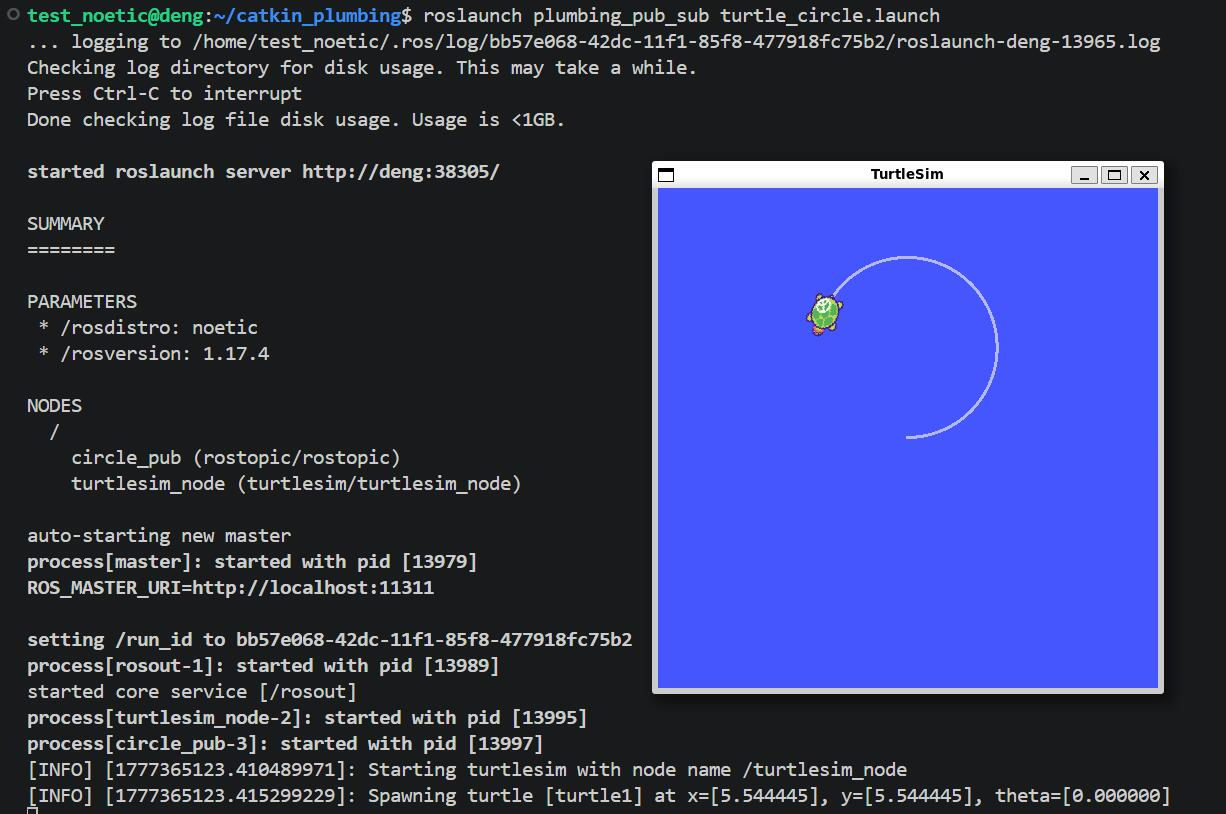
\includegraphics[width=0.55\linewidth]{results_5.PNG}
  \caption{用 launch 文件启动 turtlesim 与速度发布节点后小乌龟开始作圆周运动。}
  \label{fig:turtle-launch}
\end{figure}

仅看到圆形并不足以验证仿真状态，所以我们又订阅了 \verb|/turtle1/pose|。这个话题由 turtlesim 内部以高频率发布，包含 $x$、$y$、$\theta$、\verb|linear_velocity|、\verb|angular_velocity| 五个字段。订阅节点收到后将这些值打印出来，可以看到 $x$、$y$ 在持续变化、$\theta$ 均匀增加、线速度与角速度稳定在我们设定的数值附近，这与圆周运动的运动学特征完全一致。

\begin{figure}[htbp]
  \centering
  \begin{subfigure}{0.42\linewidth}
    \centering
    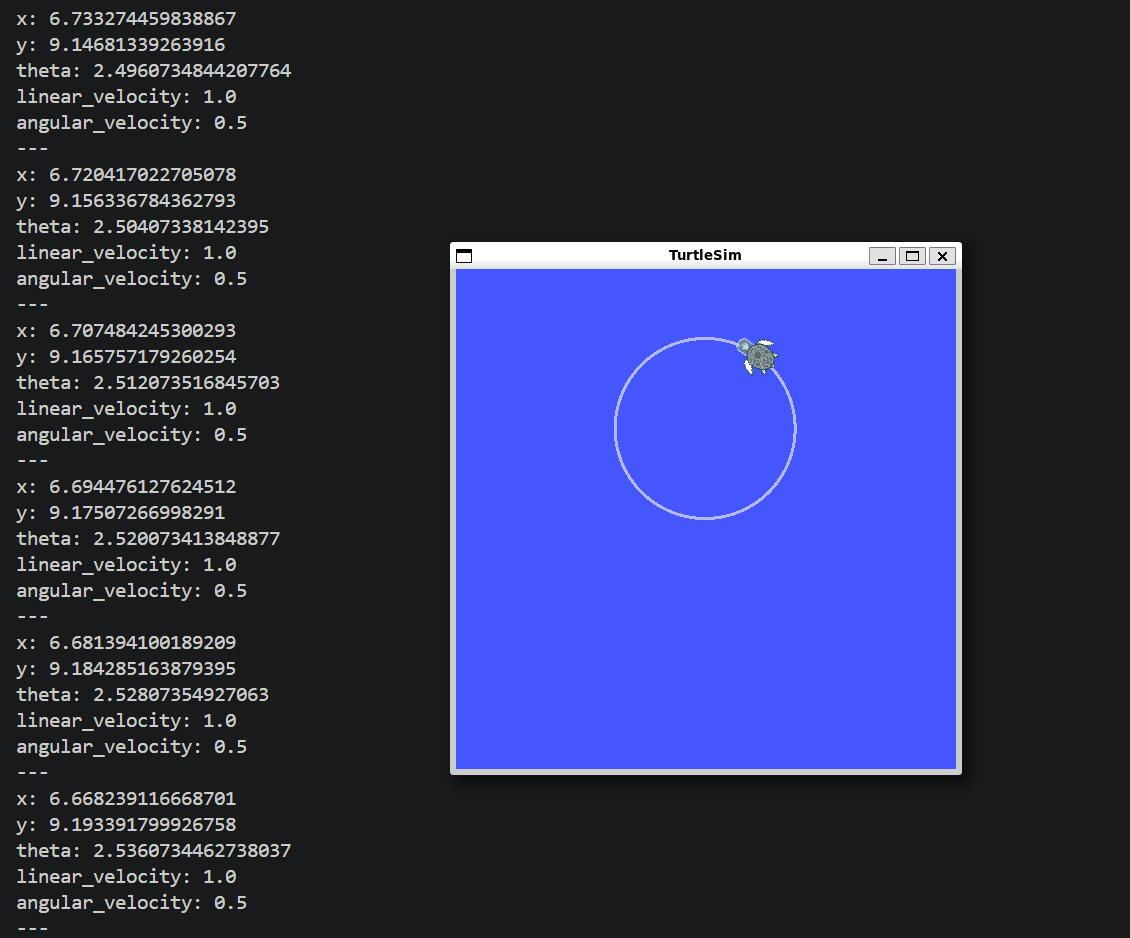
\includegraphics[width=\linewidth]{results_10.PNG}
    \caption{圆周运动与位姿输出}
    \label{fig:turtle-pose}
  \end{subfigure}
  \hfill
  \begin{subfigure}{0.42\linewidth}
    \centering
    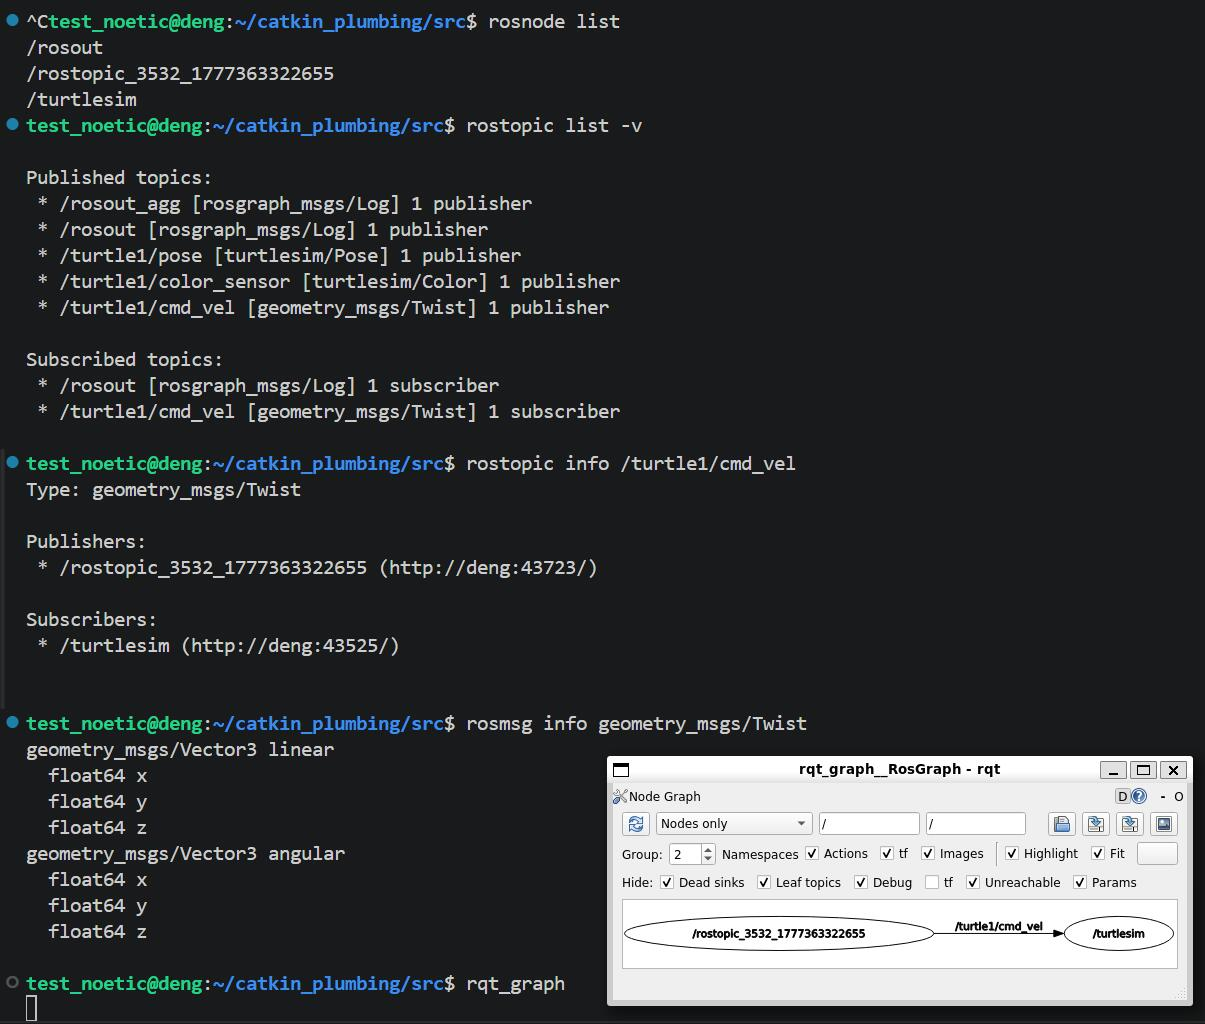
\includegraphics[width=\linewidth]{results_9.PNG}
    \caption{节点、话题与 rqt\_graph}
    \label{fig:turtle-graph}
  \end{subfigure}
  \caption{小乌龟实验中位姿反馈与节点关系图。}
  \label{fig:turtle-pose-graph}
\end{figure}

为了从计算图层面进一步验证整个系统的连接关系，我们用 \verb|rosnode list| 查看活动节点、用 \verb|rostopic list -v| 列出话题及其订阅发布情况、用 \verb|rostopic info /turtle1/cmd_vel| 查看具体话题的拓扑、再用 \verb|rosmsg info geometry_msgs/Twist| 查看消息字段。这些信息合起来就构成 ROS 计算图的完整描述。\verb|rqt_graph| 是它的可视化版本，从图 \ref{fig:turtle-graph} 可以清楚看到 \verb|circle_pub| 节点通过 \verb|/turtle1/cmd_vel| 把速度指令传给 \verb|turtlesim_node|，节点之间是松耦合的，连接关系完全由话题名定义。

\subsection{话题通信实验}

话题通信采用的是发布/订阅模式。发布方不需要知道有谁在订阅，只是把消息扔到指定话题上；订阅方也不必关心是谁发布的，只要订阅同名话题就能在回调中收到数据。这种解耦特性非常适合传感器数据、速度命令、状态广播之类的连续数据流。

\subsubsection{发布者}

发布者节点初始化时使用名字 \verb|talker_py|，向 \verb|chatter| 话题发布 \verb|std_msgs/String| 类型的消息。循环频率由 \verb|rospy.Rate(10)| 控制，意味着每秒大约执行 10 次循环、发出 10 条消息。每条消息的内容是字符串 \verb|Hello ROS Python| 加上自增的整数计数，发布之后同时打印到终端日志里方便观察。

\subsubsection{订阅者}

订阅者节点叫 \verb|listener_py|，使用 \verb|rospy.Subscriber| 订阅 \verb|chatter| 话题，并指定回调函数读取 \verb|msg.data| 字段。从图 \ref{fig:sub-py} 可以看到，订阅终端持续打印"我听见：Hello ROS Python ..."，与发布端的内容完全对应。由于发布频率为 10 Hz，订阅端的输出节奏也大致是 0.1 秒一行，二者频率上保持一致。

\begin{figure}[htbp]
  \centering
  \begin{subfigure}{0.42\linewidth}
    \centering
    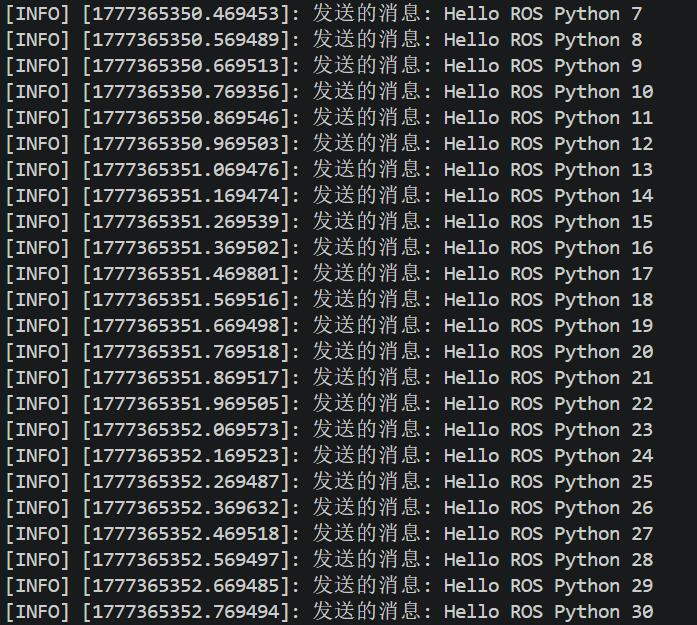
\includegraphics[width=\linewidth]{results_4.PNG}
    \caption{发布者节点以 10 Hz 发出消息}
    \label{fig:pub-py}
  \end{subfigure}
  \hfill
  \begin{subfigure}{0.42\linewidth}
    \centering
    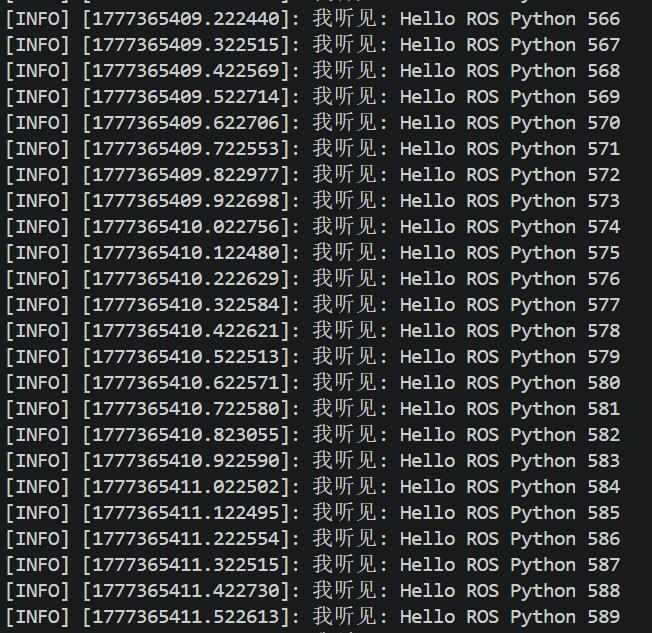
\includegraphics[width=\linewidth]{results_3.PNG}
    \caption{订阅者节点接收并打印}
    \label{fig:sub-py}
  \end{subfigure}
  \caption{话题通信中发布与订阅节点的运行结果。}
  \label{fig:pubsub-py}
\end{figure}

为了再现"多节点一键启动"的工作方式，我们还为这一对节点写了 launch 文件。运行 \verb|roslaunch| 之后，终端先打印节点摘要，然后发布与订阅日志开始交替出现，这说明两个节点已经被同一个 launch 文件托管并在同一个 ROS Master 下完成了通信。

\begin{figure}[htbp]
  \centering
  \begin{subfigure}{0.42\linewidth}
    \centering
    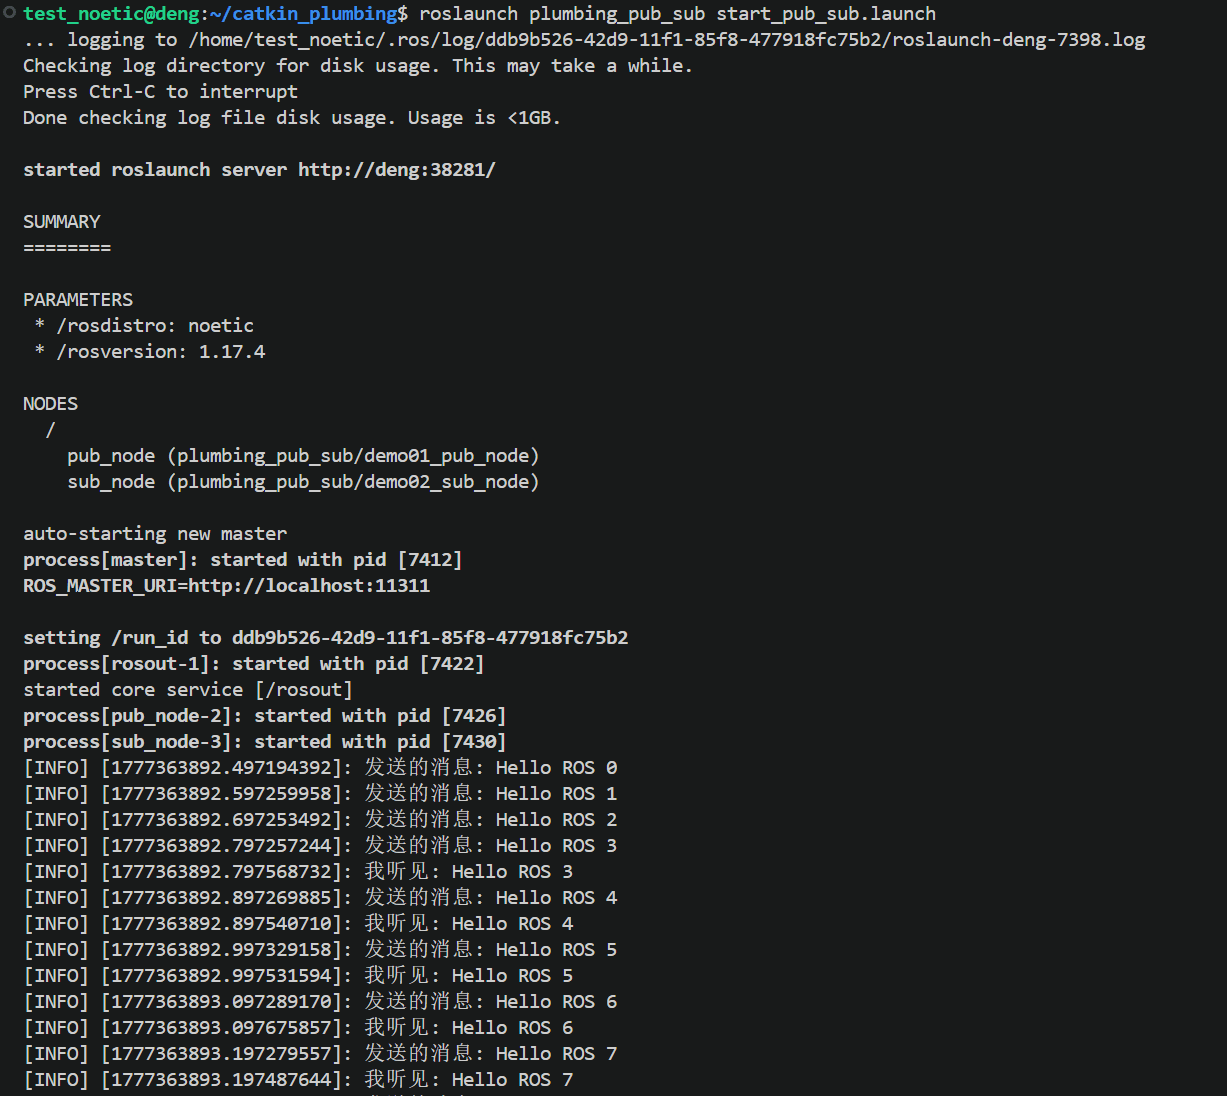
\includegraphics[width=\linewidth]{results_7.PNG}
    \caption{用 launch 启动发布订阅节点}
    \label{fig:pubsub-launch}
  \end{subfigure}
  \hfill
  \begin{subfigure}{0.42\linewidth}
    \centering
    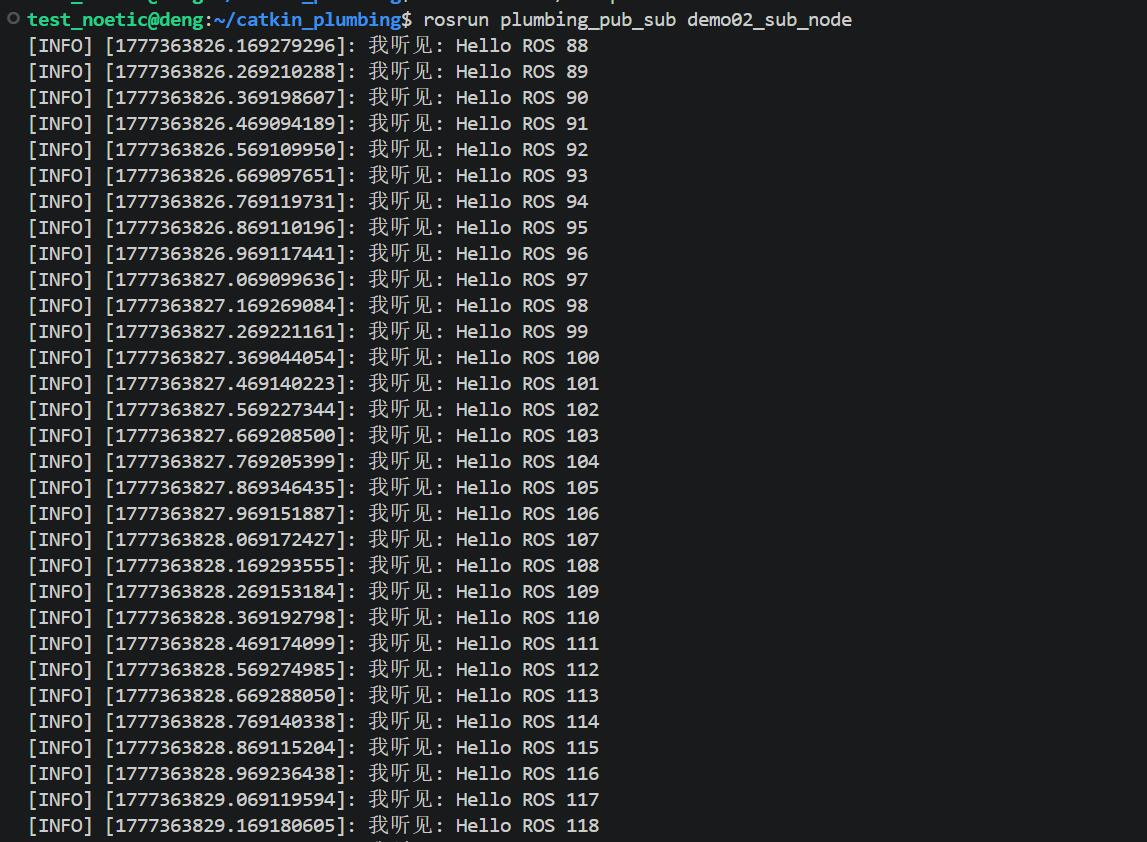
\includegraphics[width=\linewidth]{results_8.PNG}
    \caption{单独运行的订阅节点接收消息}
    \label{fig:sub-alone}
  \end{subfigure}
  \caption{发布订阅实验在 launch 启动与单独运行下的结果。}
  \label{fig:pubsub-launch-alone}
\end{figure}

值得指出的是，订阅节点不论是用 \verb|rosrun| 单独启动还是被 launch 文件一起拉起来，只要订阅的话题名一致就能正常收到数据。这正是话题通信灵活性的体现：节点之间靠话题名约定耦合，与启动方式无关。

\subsection{服务通信实验}

服务通信和话题通信最大的区别在于它是同步的——客户端发起请求后会阻塞，等服务端处理完返回结果才继续往下走。本实验我们自定义了一个 \verb|AddInts| 服务，请求字段是 \verb|num1| 和 \verb|num2| 两个整数，响应字段是它们的和 \verb|sum|。

服务端节点 \verb|addints_server_py| 启动后用 \verb|rospy.Service("AddInts_py", AddInts, handle)| 注册服务并阻塞等待请求。处理回调 \verb|handle| 收到请求后，先打印两个数据，然后做合法性判断：如果有负数就记录错误日志并返回默认响应，否则返回二者之和。从图 \ref{fig:server-py} 可以看到服务端正确接收到了 10 和 20 的请求。

客户端 \verb|addints_client_py| 在调用之前先用 \verb|rospy.wait_for_service("AddInts_py")| 等待服务出现，再用 \verb|rospy.ServiceProxy| 创建一个服务代理。这种"先等再调"的写法避免了启动顺序错乱导致的失败：即便客户端跑起来时服务端还没注册完毕，客户端也只是阻塞等待而不会立刻报错。客户端提交 10 和 20 之后收到了 30，整个调用链路完整跑通（图 \ref{fig:client-py}）。

\begin{figure}[htbp]
  \centering
  \begin{subfigure}{0.42\linewidth}
    \centering
    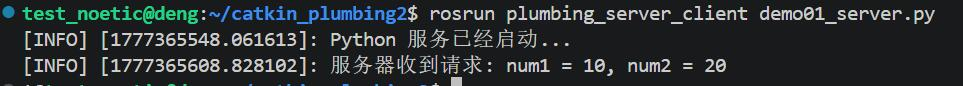
\includegraphics[width=\linewidth]{results_1.PNG}
    \caption{服务端收到 10 与 20}
    \label{fig:server-py}
  \end{subfigure}
  \hfill
  \begin{subfigure}{0.42\linewidth}
    \centering
    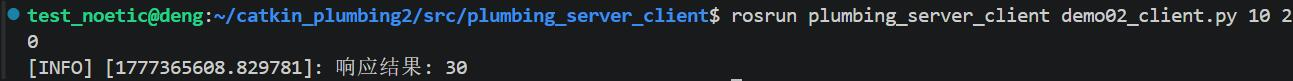
\includegraphics[width=\linewidth]{results_2.PNG}
    \caption{客户端取到求和结果 30}
    \label{fig:client-py}
  \end{subfigure}
  \caption{服务通信中服务端与客户端的运行结果。}
  \label{fig:service-py}
\end{figure}

除了 Python 实现，我们也在课程参考代码上跑了一遍 C++ 版本的服务通信，命令行结果同样显示"请求正常处理，响应结果：30"（图 \ref{fig:service-basic}）。两种语言下结果一致，再次说明服务通信的契约只取决于服务名和服务类型——对调用方而言，背后用什么语言实现并不影响最终结果。

\begin{figure}[htbp]
  \centering
  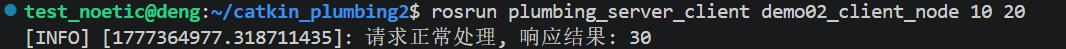
\includegraphics[width=0.6\linewidth]{results_6.PNG}
  \caption{基本服务通信实验中客户端发送 10 与 20，服务端返回 30。}
  \label{fig:service-basic}
\end{figure}

\subsection{launch 文件实验}

当一次实验涉及多个节点时，逐个用 \verb|rosrun| 启动既容易遗漏也不便于复现。launch 文件就是为了解决这件事——它用 XML 把要启动的节点、参数和命名规则全部写下来，再交给 \verb|roslaunch| 统一管理。本实验分别为小乌龟仿真和发布订阅写了 launch 文件。

小乌龟实验的 launch 同时启动 \verb|turtlesim_node| 和 \verb|circle_pub| 两个节点。\verb|roslaunch| 检测到没有正在运行的 master 时会先自启动一个 roscore，然后按照 launch 顺序拉起两个节点；只要仿真窗口出现，小乌龟立刻开始画圆。发布订阅实验的 launch 也是类似——发布者打印"发送的消息"、订阅者打印"我听见"，两条日志在终端中交替出现，一目了然地说明它们被绑定到了同一个 ROS 计算图里。

\section{结论}

通过本次实验我们认识到，ROS 中节点之间的协作并不依赖代码层面的直接调用，而是依靠注册中心（Master）和统一的通信图。话题通信支撑了 \verb|chatter| 字符串收发、turtlesim 的速度控制和位姿订阅，这些场景都体现了它在连续数据流上的优势；服务通信支撑了 \verb|AddInts| 整数求和，体现的是它一次调用一次返回的同步特性；launch 文件则把多节点的启动过程一次性固化下来，方便实验复现和分发。

从运行结果可以看出，只要话题名、服务名和消息类型对得上，节点用 \verb|rosrun| 单独启动还是 \verb|roslaunch| 一并启动都能正常通信，节点的语言（Python 或 C++）也不影响最终结果。这次实验完成了从单节点编写到多节点协作的过渡，也为后续做更复杂的机器人系统打好了基础。

\section{问题讨论}

\textbf{节点命名、launch 命名与编译目标命名的区别。} \verb|init_node()| 中传入的字符串是节点向 Master 注册的运行期名称，\verb|rosnode list|、\verb|rqt_graph| 看到的都是它。launch 文件 \verb|<node>| 标签里的 \verb|name| 同样是运行期名，但由 \verb|roslaunch| 在启动时统一指定，会覆盖代码里的默认值，便于同一份代码在不同 launch 中被赋予不同节点名。CMakeLists.txt 里 \verb|add_executable| 中的名字属于编译层面，只决定生成哪个可执行文件，\verb|rosrun| 用它定位二进制，本身不是计算图中的节点名。

\textbf{一个功能包可以包含多少节点。} 没有数量限制：发布者、订阅者、服务端、客户端可以共存在同一个包里，本实验的发布订阅包和服务包都包含两个节点。实际开发中更看重组织合理性——把功能无关的节点塞进同一个包虽然能编过，但维护和依赖都会变乱，更常见的做法是按"一组紧密相关的功能"划分包的边界。

\textbf{roslaunch 是否需要提前启动 roscore。} 多数情况下不需要。\verb|roslaunch| 启动时会找当前可用的 Master，找不到就自动拉起一个新的 roscore；如果系统里已经有正在运行的 master 或显式设置了 \verb|ROS_MASTER_URI|，则连接到对应实例而不会重复启动。手动跑 \verb|roscore| 仍可行，只是非必需。

\textbf{话题自定义消息与服务自定义消息的比较。} 话题消息保存在 \verb|.msg| 文件里，描述一种单向数据流的结构，发送方不关心接收方是否处理完，适合传感器数据、位姿、控制指令的连续输出。服务消息保存在 \verb|.srv| 文件里，用 \verb|---| 分成请求和响应两块，描述一次调用的输入输出关系，本质上更像远程函数调用。

\textbf{为什么 CMakeLists.txt 中需要 add\_dependencies()。} 功能包里一旦使用了自定义消息或服务，构建过程必须先把 \verb|.msg|/\verb|.srv| 转成对应语言的代码（C++ 是头文件如 \verb|AddInts.h|）。如果可执行目标在头文件未生成时就开始编译，会报"找不到头文件"。\verb|add_dependencies()| 的作用就是显式约束编译顺序，它不改变程序逻辑。Python 节点因为 \verb|rospy| 在运行期动态导入消息模块，不存在这种依赖。

\textbf{先启动客户端再启动服务端的问题。} 客户端启动后立即发起调用而服务端还没注册，同步调用会因 Master 上找不到提供者而失败。解决方法有两种：按顺序启动，或在客户端代码里加等待逻辑（C++ 用 \verb|ros::service::waitForService()|，Python 用 \verb|rospy.wait_for_service()|），本实验客户端采用了后者。如果服务端始终未起，客户端会一直阻塞除非设超时；服务端崩溃后再次调用会抛异常，需要异常捕获并决定是否重试。类似思路也体现在话题通信的 \verb|queue_size| 上——队列太小丢老消息，太大增加延迟。最后，\verb|rospy.spin()| 适合"被动等待回调"的订阅者和服务端，\verb|while not rospy.is_shutdown()| 更适合"主动周期性执行"的发布者。

\end{document}
